\section{Text classification using
BERT}\label{text-classification-using-bert}

In this notebook, we will utilize a pre-trained deep learning model to
analyze some text. The model's output will be used to categorize the
text, which is a collection of sentences extracted from movie reviews.
Our goal is to determine whether each sentence conveys a positive or
negative sentiment towards the subject.

\paragraph{Objective}\label{objective}

Our objective is to develop a model that can analyze a given sentence
and determine whether it expresses a positive sentiment, in which case
it should produce a value of 1, or a negative sentiment.

The model comprises two components:
\href{https://huggingface.co/transformers/model_doc/distilbert.html}{DistilBERT} and a basic \href{https://scikit-learn.org/stable/modules/generated/sklearn.linear_model.LogisticRegression.html}{Logistic Regression} model from scikit-learn.

\begin{itemize}
\item DistilBERT processes the input sentence and passes on relevant
  information to the Logistic Regression model for sentiment
  classification. It is a lighter and faster version of BERT that
  performs comparably well.
\item The data shared between the two models is a vector of size 768. This
  is because DistilBERT represents each input sentence as a sequence of
  vectors, with each vector having a size of 768. This vector sequence
  is then fed to the Logistic Regression model for classification.
\end{itemize}

\paragraph{Dataset - SST2}\label{dataset---sst2}

The SST2 dataset is a widely-used benchmark dataset for sentiment
analysis and text classification tasks. It consists of movie reviews
from Rotten Tomatoes, with each review labeled as positive or negative.
The dataset contains 11,855 training sentences and 2,210 testing
sentences, each of which is parsed into a binary parse tree to capture
its grammatical structure. The dataset has been used to evaluate the
performance of various natural language processing models, including
BERT and its variants. You can find the dataset
\href{https://nlp.stanford.edu/sentiment/index.html}{here}.

\begin{lstlisting}[language=Python]
import numpy as np
import pandas as pd
from sklearn.model_selection import train_test_split, GridSearchCV, cross_val_score
from sklearn.linear_model import LogisticRegression
import torch
import transformers
\end{lstlisting}

\subsubsection{Import the dataset}\label{import-the-dataset}

\begin{lstlisting}[language=Python]
url = 'https://github.com/clairett/pytorch-sentiment-classification/raw/master/data/SST2/train.tsv'
df = pd.read_csv(url, delimiter='\t', header=None, nrows=2500)
df.head()
\end{lstlisting}

\begin{table}
    \centering
    \begin{tabular}{ccc}
          & 0 & 1 \\
          \hline
        0 & a stirring , funny and finally transporting re\ldots{} & 1\\
        1 & apparently reassembled from the cutting room f\ldots{} & 0\\
        2 & they presume their audience wo n't sit still f\ldots{} & 0\\
        3 & this is a visually stunning rumination on love\ldots{} & 1\\
        4 & jonathan parker 's bartleby should have been t\ldots{} & 1\\
    \end{tabular}
\end{table}

\subsubsection{Load Pretrained model}\label{load-pretrained-model}

\begin{lstlisting}[language=Python]
# For DistilBERT:
model_class, tokenizer_class, pretrained_weights = (transformers.DistilBertModel,
                                                    transformers.DistilBertTokenizer,
                                                    'distilbert-base-uncased')

# Load pretrained model/tokenizer
tokenizer = tokenizer_class.from_pretrained(pretrained_weights)
model = model_class.from_pretrained(pretrained_weights)
\end{lstlisting}

\begin{lstlisting}
Some weights of the model checkpoint at distilbert-base-uncased were not used when initializing DistilBertModel: ['vocab_transform.bias', 'vocab_transform.weight', 'vocab_projector.weight', 'vocab_layer_norm.bias', 'vocab_layer_norm.weight', 'vocab_projector.bias']
- This IS expected if you are initializing DistilBertModel from the checkpoint of a model trained on another task or with another architecture (e.g. initializing a BertForSequenceClassification model from a BertForPreTraining model).
- This IS NOT expected if you are initializing DistilBertModel from the checkpoint of a model that you expect to be exactly identical (initializing a BertForSequenceClassification model from a BertForSequenceClassification model).
\end{lstlisting}

The code above demonstrates how to load a pre-trained DistilBERT model
and tokenizer from the Transformers library by Hugging Face, which can
be used for various natural language processing tasks. \newline

First, the \lstinline{model_class},
\lstinline{tokenizer_class}, and
\lstinline{pretrained_weights} variables are defined to
hold the appropriate classes and weights required for the
\textbf{DistilBERT} model. \newline

The \lstinline{DistilBertTokenizer} class is used to
tokenize raw text data and prepare it for input to the DistilBERT model.
The \lstinline{DistilBertModel} class is the
implementation of the DistilBERT model itself. The
\lstinline{pretrained_weights} variable is set to
\lstinline{distilbert-base-uncased}, which indicates the
specific pre-trained DistilBERT model to be used. \newline

Next, the \lstinline{tokenizer} variable is initialized
using the \lstinline{from_pretrained()} method, which
loads the pre-trained tokenizer for the specified DistilBERT model. This
allows the raw text data to be tokenized and encoded in a way that can
be understood by the model. \newline

Finally, the model variable is initialized using the
\lstinline{from_pretrained()} method, which loads the
pre-trained DistilBERT model with the specified weights. This allows the
model to be used for various NLP tasks, such as sentiment analysis or
text classification. \newline
\begin{lstlisting}[language=Python]
# tokenize all the reviews in column 0 of the dataframe "df"
tokenized = df[0].apply((lambda x: tokenizer.encode(x, add_special_tokens=True)))
\end{lstlisting}
The code above tokenizes a column of reviews in a Pandas DataFrame using
the pre-trained tokenizer from the DistilBERT model, which was
previously loaded. The resulting tokenized reviews are stored in a new
Pandas Series called \lstinline{tokenized}. \newline

First, the \lstinline{tokenizer.encode()} method is used
to encode each review in the DataFrame. The
\lstinline{encode()} method converts the text into a
sequence of integers that can be fed into the
\lstinline{DistilBERT} model. The
\lstinline{add_special_tokens=True} argument is passed
to add special tokens like \textbf{{[}CLS{]}} (beginning of sequence)
and \textbf{{[}SEP{]}} (end of sequence) to the beginning and end of
each encoded review, respectively. \newline

The \lstinline{apply()} method is used to apply the
\lstinline{tokenizer.encode()} function to each row in the
DataFrame column containing the reviews. The resulting tokenized reviews
are stored in a new Pandas Series called tokenized. \newline

\begin{lstlisting}[language=Python]
def visualized_sentence_embedding(df: pd.DataFrame, tokenized: pd.Series) -> pd.DataFrame:
    """
    Function to see tokens and embeddings of the first review in df.
    """
    tokens = df.iloc[0,0].split(" ")
    tokens.insert(0, "CLS")
    tokens.append("SEP")
    assert len(tokens) == len(tokenized[0])
    token_embeddings = list(zip(tokens, tokenized[0]))
    df_token_embeddings = pd.DataFrame(token_embeddings, columns=["Tokens", "Embeddings"])
    return df_token_embeddings
\end{lstlisting}

\begin{lstlisting}[language=Python]
df_token_embeddings = visualized_sentence_embedding(df, tokenized)
df_token_embeddings.head(10)
\end{lstlisting}

\begin{table}[!htbp]
    \centering
    \begin{tabular}{ccc}
         & Tokens & Embeddings\\
         \hline
        0 & CLS & 101\\
        1 & a & 1037\\
        2 & stirring & 18385\\
        3 & , & 1010\\
        4 & funny & 6057\\
        5 & and & 1998\\
        6 & finally & 2633\\
        7 & transporting & \textbf{}\\
        8 & re & 2128\\
        9 & imagining & \textbf{}\\
    \end{tabular}
\end{table}

\subsubsection{Padding}\label{padding}

Once the reviews in a DataFrame are tokenized, they are stored as a list
of sentences (\lstinline{tokenized}; data type
=\lstinline{pd.Series}), where each sentence is
represented as a list of tokens. In order to process these examples in
one batch using BERT, it is necessary to pad all of the lists to the
same length. This allows the input to be represented as a single
2-dimensional array, rather than a list of variable-length lists. By
doing this, the processing time can be greatly reduced.

\begin{lstlisting}[language=Python]
max_len = 0
max_len = max([len(i) for i in tokenized.values if len(i) > max_len])
padded_token_embeddings = np.array([i + [0]*(max_len-len(i)) for i in tokenized.values])
print(padded_token_embeddings.shape)
\end{lstlisting}

\begin{lstlisting}
(2500, 65)
\end{lstlisting}

The above code performs the following steps:

\begin{enumerate}
\def\labelenumi{\arabic{enumi}.}
\item
  Initializes \lstinline{max\_len} to zero.
\item
  Computes the maximum length of the tokenized reviews using a list
  comprehension that iterates over the tokenized reviews, returns their
  lengths. The resulting maximum length is assigned to the
  \lstinline{max\_len} variable.
\item
  Pads the tokenized reviews with zeros to make them all the same length
  as the maximum length \lstinline{max\_len}. This is done
  using a list comprehension that iterates over the tokenized reviews,
  appends 0 to the end of each review until it has the same length as
  \lstinline{max\_len}, and converts the resulting list of
  padded reviews to a NumPy array. The resulting padded token embeddings
  are assigned to the
  \lstinline{padded\_token\_embeddings} variable.
\item
  Overall, this code computes the maximum length of the tokenized
  reviews and pads them with zeros to make them all the same length,
  which is necessary for feeding them into a deep learning model.
\end{enumerate}

\subsubsection{Masking}\label{masking}

In order to avoid confusing BERT with the padding added to the tokenized
reviews, we need to create a separate variable called attention\_mask.
This variable indicates which tokens should be attended to by the model
and which tokens should be ignored (masked) during processing. By
setting the attention mask to 1 for the real tokens and 0 for the
padding tokens, we can tell BERT to ignore the padding when processing
the input. This helps to improve the accuracy of the model's
predictions.

\begin{lstlisting}[language=Python]
attention_mask = np.where(padded_token_embeddings != 0, 1, 0)
assert attention_mask.shape == padded_token_embeddings.shape
print(attention_mask.shape)
\end{lstlisting}

\begin{lstlisting}
(2500, 65)
\end{lstlisting}

\subsubsection{Model inputs}\label{model-inputs}

We're now ready to train a deep learning model using PyTorch. We will be
using the pre-trained \textbf{DistilBERT} model that we previously
loaded. First, we need to prepare our inputs for the model. We take our
tokenized and padded sentences and convert them into PyTorch tensors
using the \lstinline{torch.tensor()} function.

we can pass the \lstinline{input\_ids} (torch tensor) and
\lstinline{attention\_mask} tensors to the DistilBERT
model using the \lstinline{model()} function. The output
of the function, \lstinline{last\_hidden\_states}, will
contain the contextualized embeddings for each token in our input
sentences.

\begin{lstlisting}[language=Python]
input_ids = torch.tensor(padded_token_embeddings)
attention_mask = torch.tensor(attention_mask)

with torch.no_grad():
    last_hidden_states = model(input_ids, attention_mask=attention_mask)
\end{lstlisting}

\begin{lstlisting}[language=Python]
# extracting features and labels
features = last_hidden_states[0][:,0,:].numpy()
\end{lstlisting}

\textbf{Explanation for feature extraction from
\lstinline{last\_hidden\_states}:}

Suppose we have a batch of 2500 input sentences, where each sentence is
tokenized and padded to a length of 65. So, the shape of our padded
array would be (2500, 65).

Now, we pass this padded array to BERT using the
\lstinline{model()} function, and it returns a tensor
\lstinline{last\_hidden\_states} of shape (2500, 65, 768).
Here, 2500 is the batch size, 65 is the length of the padded sentence,
and 768 is the size of the BERT embedding for each token.

To get a fixed-length representation of each sentence, we take the first
token of each sentence, which is the \lstinline{[CLS]}
token. So, we extract the embeddings corresponding to the
\lstinline{[CLS]} token, which is located at index 0 in
the second dimension of last\_hidden\_states.

To get these embeddings for each sentence in the batch, we use the
slicing operation \lstinline{[:,0,:]}. This selects all
elements along the first dimension (which corresponds to the batch
size), the first element along the second dimension (which corresponds
to the \lstinline{[CLS]} token), and all elements along
the third dimension (which corresponds to the embedding size). This
returns a tensor of shape (2500, 768), where each row corresponds to the
embedding of a single sentence.

Finally, we convert this tensor to a numpy array using
\lstinline{.numpy()}, which gives us a 2D numpy array
features of shape (2500, 768), where each row represents the
fixed-length representation of a sentence.

\begin{lstlisting}[language=Python]
labels = df[1]
assert len(features) == len(labels)
\end{lstlisting}

\subsubsection{Split data into training and testing
sets}\label{split-data-into-training-and-testing-sets}

\begin{lstlisting}[language=Python]
train_features, test_features, train_labels, test_labels = train_test_split(features, labels)
\end{lstlisting}

\subsubsection{Logistic Regression}\label{logistic-regression}

\begin{lstlisting}[language=Python]
lr_clf = LogisticRegression(C=5, max_iter=1000)
lr_clf.fit(train_features, train_labels)
\end{lstlisting}

\phantomsection\label{sk-container-id-1}
In a Jupyter environment, please rerun this cell to show the HTML
representation or trust the notebook. On GitHub, the HTML representation
is unable to render, please try loading this page with nbviewer.org.

LogisticRegression

\begin{lstlisting}[language=Python]
# see how our trained LR model performs on the test set
lr_clf.score(test_features, test_labels)
\end{lstlisting}

\begin{lstlisting}
0.8336
\end{lstlisting}

\subsubsection{Further improvements}\label{further-improvements}

\begin{itemize}
\item Fine tune DistilBERT
\item  Use GridSearchCV for getting best hyperparameters for the
  LogisticRegression model.
\item  Try other classifiers, build a NN for classification, or used another
  pretrained neural network for classification.
\end{itemize}

\section{Fine-tuning BERT}
\href{https://www.youtube.com/watch?v=FyOtgrF8w_w}{Youtube}

\subsection{Steps to Finetune BERT}

\begin{enumerate}
    \item First, we need to import all the necessary packages. We will use the \href{https://pypi.org/project/datasets/}{\textbf{datasets}} library to load data and functions to compute metrics. From HuggingFace's \href{https://pypi.org/project/transformers/}{\textbf{transformers}} package, we will import tokenizers, trainers, and models for sentence classification.
    \begin{lstlisting}
from datasets import load_dataset
from transformers import AutoTokenizer
from transformers import AutoModelForSequenceClassification
from transformers import TrainingArguments, Trainer
import numpy as np
from datasets import load_metric
    \end{lstlisting}
    \item Next, we will define some functions to compute our metrics and tokenize our sentences.
    \begin{lstlisting}
def compute_metrics(eval_pred):
    logits, labels = eval_pred
    predictions = np.argmax(logits, axis=-1)
    return metric.compute(predictions=predictions, references=labels)

def tokenize_function(examples):
    return tokenizer(examples["text"], padding="max_length", truncation=True)
    \end{lstlisting}
    \item Now, we can load and preprocess our dataset. Remember that we will use the \lstinline|datasets| package to load data. The \lstinline|datasets| package has many inbuilt datasets available, and you can find a list \href{https://huggingface.co/datasets}{\textbf{here}}.
    \item The tokenizer we select needs to be the same as the model we are using. There are many pre-trained models available in \lstinline|transformers| and you can find a list of them \href{https://huggingface.co/transformers/pretrained_models.html}{\textbf{here}}. In the code below, you can see that I am using the \lstinline|bert-base-cased| model. Once we have selected the model, we need to tokenize our dataset. I have also added code to use a small subset of the data to make training faster. However, you may choose to use the whole dataset by uncommenting the last two lines.
    \begin{lstlisting}
tokenizer = AutoTokenizer.from_pretrained("bert-base-cased")
tokenized_datasets = raw_datasets.map(tokenize_function, batched=True)

small_train_dataset = tokenized_datasets["train"].shuffle(seed=42).select(range(1000))
small_eval_dataset = tokenized_datasets["test"].shuffle(seed=42).select(range(1000))
# full_train_dataset = tokenized_datasets["train"]
# full_eval_dataset = tokenized_datasets["test"]
    \end{lstlisting}
    \item Now that we have written our data preprocessing code, we can download our model and start to train it. We will use the \lstinline|AutoModelForSequenceClassification| API to fetch the pre-trained \lstinline{bert-base-cased} model. We also need to specify the number of classes in our data.
\end{enumerate}
Finally, we can train and evaluate the model using a \lstinline|Trainer| object.

\begin{lstlisting}
model = AutoModelForSequenceClassification.from_pretrained("bert-base-cased", num_labels=<your labels>)

metric = load_metric("accuracy")

training_args = TrainingArguments("test_trainer", evaluation_strategy="epoch")

trainer = Trainer(
    model=model,
    args=training_args,
    train_dataset=small_train_dataset,
    eval_dataset=small_eval_dataset,
    compute_metrics=compute_metrics,
)
trainer.train()
trainer.evaluate()
\end{lstlisting}

\begin{quote}
Note: Fine tuning BERT takes a long time (even on GPUs), hence we are not providing a workspace for this demo. Please try this on your local machine.
\end{quote}

\section{GPT}

GPT, or Generative Pre-trained Transformer, is an advanced \href{https://en.wikipedia.org/wiki/Autoregressive_model}{\textbf{autoregressive}} language model built on the transformer architecture, which leverages self-attention mechanisms for efficiently handling long-range dependencies in sequence data. The primary goal of GPT models is to predict the next token in a given sequence by learning a probability distribution over a vast vocabulary. This is achieved through unsupervised pre-training on large-scale text corpora, followed by fine-tuning on specific tasks to generate human-like text, perform translation, answer questions, and more. \newline

The evolution of GPT began with GPT-1, which demonstrated the potential of unsupervised pre-training followed by task-specific fine-tuning. GPT-2, the successor, utilized a much larger dataset and model size, leading to substantially improved performance across various NLP tasks. However, its release was initially limited due to concerns about potential misuse. GPT-3 took the concept further, scaling up to 175 billion parameters and introducing the "\href{https://paperswithcode.com/task/few-shot-learning}{\textbf{few-shot learning}}" paradigm, which allowed the model to perform tasks with very limited task-specific training data.\newline

GPT-4 builds upon the advancements of its predecessors, featuring an even larger model size and enhanced pre-training techniques. This latest iteration benefits from architectural improvements, such as sparsity and attention mechanisms that facilitate more efficient training and inference. GPT-4's greater capacity enables it to learn more sophisticated language patterns and generate higher-quality output across a broader range of tasks. Additionally, GPT-4 can be fine-tuned with smaller datasets, making it a powerful tool for specialized applications in various domains. Despite its impressive capabilities, GPT-4 still faces challenges in controlling generated content, ensuring factual accuracy, and mitigating biases present in training data.

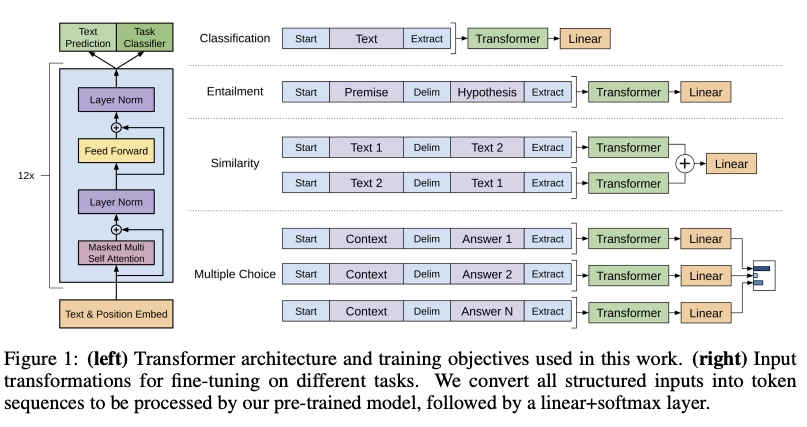
\includegraphics[width=1\linewidth]{img//rnn//transformers/cleanshot-2023-04-16-at-23.39.34.jpeg}
\captionof{figure}{Source: \href{https://s3-us-west-2.amazonaws.com/openai-assets/research-covers/language-unsupervised/language_understanding_paper.pdf}{\textbf{Improving Language Understanding by Generative Pre-Training}})}

\section{Text Generation using pre-trained HuggingFace Transformer
models}\label{text-generation-using-pre-trained-huggingface-transformer-models}

\subsection{Step 1: Load the pre-trained GPT-2
model}\label{step-1-load-the-pre-trained-gpt-2-model}

\begin{lstlisting}[language=Python]
from transformers import GPT2LMHeadModel, GPT2Tokenizer

# Load pre-trained GPT-2 model and tokenizer
model_name = "gpt2"
model = GPT2LMHeadModel.from_pretrained(model_name)
tokenizer = GPT2Tokenizer.from_pretrained(model_name)
\end{lstlisting}

\begin{lstlisting}
/opt/venv/lib/python3.10/site-packages/tqdm/auto.py:21: TqdmWarning: IProgress not found. Please update jupyter and ipywidgets. See https://ipywidgets.readthedocs.io/en/stable/user_install.html
  from .autonotebook import tqdm as notebook_tqdm
\end{lstlisting}

\subsection{Step 2: Define the prompt
text}\label{step-2-define-the-prompt-text}

\begin{lstlisting}[language=Python]
# Define the prompt text
prompt = "The quick brown fox"
\end{lstlisting}

\subsection{Step 3: Generate text using the GPT-2
model}\label{step-3-generate-text-using-the-gpt-2-model}

\begin{lstlisting}[language=Python]
# Generate text using the GPT-2 model
input_ids = tokenizer.encode(prompt, return_tensors="pt")
output = model.generate(input_ids, max_length=50, do_sample=True)

# Decode the generated text
generated_text = tokenizer.decode(output[0], skip_special_tokens=True)
print(generated_text)
\end{lstlisting}

\begin{lstlisting}
The attention mask and the pad token id were not set. As a consequence, you may observe unexpected behavior. Please pass your input's `attention_mask` to obtain reliable results.
Setting `pad_token_id` to `eos_token_id`:50256 for open-end generation.


The quick brown foxes, a new species and then some, are the same from year to year.

That's why some of the latest sightings are often the same.

"We can see all kinds of people, you can hear
\end{lstlisting}

In this example, we used the pre-trained GPT-2 model to generate text
based on a prompt. We first loaded the model and tokenizer using the
Hugging Face Transformers library. Then, we defined the prompt text that
we want the model to generate text from. Finally, we used the
\lstinline{generate()} method to generate text from the
prompt and decode the generated text using the tokenizer. \newline

Note that the \lstinline{generate()} method takes several
arguments, including \lstinline{max_length}, which
controls the maximum length of the generated text, and
\lstinline{do_sample}, which enables sampling from the
model distribution to generate diverse outputs. \newline

This is just a simple example of text generation using the Hugging Face
Transformers library. With this powerful library, you can explore a wide
range of models and tasks in NLP, from language translation to question
answering and beyond. \newline

TODO:

Try
\href{https://huggingface.co/models?pipeline_tag=text-generation&sort=downloads}{other
text generation models} from HuggingFace with different prompts.

\begin{lstlisting}[language=Python]
from transformers import pipeline

generator = pipeline('text-generation', model="facebook/opt-125m")
generator(prompt)
\end{lstlisting}

\begin{lstlisting}
[{'generated_text': "The quick brown fox is a good one.\nI've been using it for a while now."}]
\end{lstlisting}
